\documentclass[10pt,letterpaper]{article}
\usepackage[margin=0.85in]{geometry}
\usepackage{amsmath,amssymb,amsthm,booktabs,array,xcolor,listings,hyperref}
\usepackage{tikz,pgfplots}
\usepackage{placeins}
\pgfplotsset{compat=1.18}
\hypersetup{colorlinks=true,linkcolor=black,citecolor=black,urlcolor=blue}
\lstset{basicstyle=\ttfamily\footnotesize,breaklines=true,columns=fullflexible,keepspaces=true,showstringspaces=false,frame=single,rulecolor=\color{black!20}}
\setlength{\parskip}{4pt}
\setlength{\parindent}{0pt}
\newtheorem{proposition}{Proposition}
\title{Auditing Selective Workspace Repair\\When Provenance Is Incomplete}
\author{Fei Lin\\Manor AI}
\date{October 14, 2026\\\small Research preprint, version 0.1; not peer reviewed}
\begin{document}
\maketitle
\begin{abstract}
Selective repair reuses unaffected work after source information changes, but observed provenance may omit relevant relationships or retain incorrect ones. We study checking outside that graph, separating heuristic discovery from a statistical release condition. A frozen executable-claim benchmark contains 360 generated base workspaces, four coupled provenance conditions and eight policies. Five policies use matched 36-call inspection budgets; a ranked excluded-pool audit adds full inspection when a known finite-population count bound fails. Across 1,440 workspace-condition instances, this gate averages 59.08 calls versus 64 for full inspection, saving 7.69\%. It triggers 1,187 fallbacks and yields six releases above the configured six-claim residual tolerance. Its 90.69\% all-current frequency is below the exact full-inspection diagnostic's 100\%. A complete replay is byte-identical. The contribution is a reproducible composition study, not new statistical theory or demonstrated language-model repair superiority. Validation and patches are idealized; actual model feasibility and production-integration limits are reported explicitly.
\end{abstract}
\textbf{Keywords:} AI workspaces; provenance; selective repair; validation budgets; finite-population auditing.

\section{Problem and motivation}
A workspace can retain a report, an allocation table and an operational summary after the underlying budget changes. Updating the source does not automatically update every dependent output. Conversely, regenerating every artifact consumes resources and can disturb valid work. Selective repair therefore needs to decide which retained outputs to inspect, which to change and when the remaining uncertainty is acceptable.

An observed citation graph is useful but incomplete evidence. A missing edge can hide an affected output. An incorrect edge can waste an inspection. Even a complete influence graph can overstate actual revision obligations: a source change can cancel algebraically, remain below a rounding threshold, or leave an independently bounded value unchanged. We distinguish structural influence from the value changes that require repair in the benchmark.

Manor motivates this setting because it combines persistent tasks, shared knowledge, generated artifacts and human approval. The current study is an independent research implementation, not a deployed Manor feature. Existing artifact identities, version fields and delivery checks are plausible integration interfaces; their existence does not establish complete provenance or a working repair controller.

The research question is narrow: under incomplete or incorrect observed provenance, what residual errors remain at a fixed inspection budget, and what additional cost is incurred by a declared excluded-pool audit and fallback rule? We do not claim a new dependency algorithm or statistical confidence bound. We also do not equate a bounded count of stale claims with a completely correct business deliverable.

\section{Prior work and contribution boundary}
CodePlan combines dependency analysis, change-impact analysis and adaptive planning for repository edits~\cite{codeplan}. LEDGER already uses typed dependencies, counterfactual language-model testing and consistency checks for document editing~\cite{ledger}. MemoRepair studies invalidated sources, withdrawal of derived artifacts, validated successors and cascade repair, including the consequences of missing provenance~\cite{memorepair}. BoardroomAI performs dependency-aware selective repair and explicitly tests missing edges~\cite{boardroom}. CAVERT concerns execution consistency and the evidence needed to diagnose and recover agent workflows~\cite{cavert}.

Excluded-pool auditing, exact finite-population confidence bounds, and planned sequential selective-release audits also have direct precedents~\cite{coverage,selective}. We use a single planned look rather than introducing a new sequential procedure. Our contributions are: an executable benchmark separating observed lineage from actual value-delta obligations; a matched-cost comparison of graph, lexical, random and hybrid inspection policies; and a composition of ranked discovery, known auditing and explicit fallback whose residual-count interpretation can be checked from raw records. These contributions are bounded systems evidence, not demonstrated superiority over the full implementations of LEDGER or MemoRepair.

\section{Frozen-state repair contract}
Let a frozen workspace contain sources $S^0$, updated sources $S^1$, and $m$ retained claim blocks $a_i^0$. A deterministic reference program $f_i$ defines the target value of each block. Its reference target is
\begin{equation}
a_i^\star=f_i(S^1),\qquad
y_i=\mathbf{1}[a_i^0\ne a_i^\star].
\end{equation}
The hidden set $A=\{i:y_i=1\}$ contains actual revision obligations. It is held by the evaluator, not supplied to inspection policies. The observed graph $\widehat G$ contains retained citations and is allowed to miss or add edges. In general,
\begin{equation}
\mathrm{Desc}_{\widehat G}(\Delta S)\ne A.
\end{equation}
Even the complete influence graph need not identify exactly $A$: $b-b$ remains zero after $b$ changes. This benchmark's targets are fixed functions of the updated sources; inspecting and patching one claim cannot change another claim's target.

A validation call reveals whether one selected block is stale and, when it is, replaces only its generated block with the reference target. Every call is charged, including a repeated call. All evaluated policies avoid repeats. Protected human notes are outside the patch operation for every policy. This is structural preservation by design, not evidence that conflicting human edits can be resolved semantically.

Let $I$ be the inspected set. The final residual count and inspection fraction are
\begin{equation}
L(I)=|A\setminus I|,\qquad C(I)=|I|/m.
\end{equation}
We separately report $\mathbf{1}[L(I)=0]$ and the fraction of initial obligations repaired. The first is a stringent workspace-instance measure. Neither is a model reasoning score, a token cost, or a measure of real-world financial risk.

\section{Discovery followed by a planned audit}
The ranked-audit policy first inspects $d=12$ claims using public-only signals. The remaining pool $U$ is then frozen, with size $N=m-d=52$. It draws $n=24$ claims uniformly without replacement, observes $k$ stale claims, and repairs detected claims. The sample order is fixed by a seed independent of the hidden labels.

For an unknown stale count $K$ in $U$, the sample-positive count has distribution
\begin{equation}
\Pr_K(X=x)=\frac{\binom Kx\binom{N-K}{n-x}}{\binom Nn}.
\end{equation}
Using the established one-sided exact inversion, define
\begin{equation}\label{eq:bound}
K^+(N,n,k;\delta)=\max\left\{K\in[k,N-n+k]:
 \sum_{x=\max(0,n-N+K)}^{\min(k,n,K)}\Pr_K(X=x)>\delta\right\}.
\end{equation}
The count bound for uninspected stale blocks is $B=K^+-k$. The fixed policy uses $\delta=0.05$ and tolerates at most
\begin{equation}\label{eq:gate}
\tau=\lfloor 0.10m\rfloor=6.
\end{equation}
It stops when $B\le\tau$; otherwise it inspects the remaining blocks. There is exactly one audit look per instance, with no repeated confidence testing until a favorable outcome occurs.

\begin{proposition}[Residual-count control under fixed-state assumptions]
For a fixed workspace and exact validation labels, suppose the audit is a uniform sample of the frozen remaining pool. The policy's probability of stopping with more than $\tau$ stale uninspected blocks is at most $\delta$. With an exact validator, a completed full-inspection fallback has zero residual stale blocks.
\end{proposition}
\begin{proof}
The known exact upper bound satisfies $\Pr(K>K^+)\le\delta$. If $K\le K^+$, repairing the $k$ sample positives leaves at most $K^+-k=B$ stale blocks outside the sample. Stopping requires $B\le\tau$. An unsafe stop therefore implies the confidence-bound failure event. Full inspection visits and patches every remaining stale block under the exact reference validator.
\end{proof}
This argument applies per frozen instance, unconditionally over the prespecified audit randomization. It does not assert $\Pr(L\le\tau\mid\text{gate passes})\ge0.95$. It is not a simultaneous 95\% guarantee over the entire corpus, and a permitted residual of six is not zero-error certification. Labels must remain fixed: a source update, semantic patch that changes another target, or unvalidated version change invalidates the argument. A semantic validator with false negatives does not inherit the guarantee without additional assumptions.

There is an unavoidable cost to stricter claims. If no positives are observed and one missed stale block would be unacceptable, then for $K=1$,
\begin{equation}
\Pr(X=0\mid K=1)=(N-n)/N.
\end{equation}
Excluding that possibility at $\delta=0.05$ requires $n/N\ge0.95$ under the strict-tail convention in Equation~\ref{eq:bound}. Large savings and distribution-free zero-miss certification cannot both be obtained by a small random audit alone.

\section{Executable study design}
\subsection{Data and independence}
The protocol, code hash and all generated cases were frozen before held-out execution. This is a local recorded freeze, not external preregistration. There are three parameterized families: budget, capacity and pricing. Each has 120 base workspaces, giving 360 generated base workspaces. Every workspace has 64 claim blocks and one changed scalar source. Four coupled true-edge deletion probabilities, 0\%, 10\%, 30\% and 50\%, produce 1,440 workspace-condition instances. Realized missing-edge fractions vary by instance. The same base facts, expressions and source update are reused across conditions; these are not 1,440 independent business tasks.

Reference programs include direct sources, scaling, arithmetic, rounding, minimum and maximum operations. They therefore distinguish influence from actual value changes. Incorrect citations are inserted with probability 0.05 per claim, fixed across missing-edge conditions; the 0\% missing-edge condition can still contain incorrect edges. Claim IDs and public order are randomized. Titles follow generated operand topics with 30\% lexical masking, which creates a synthetic relevance signal. Consequently, lexical ranking results cannot establish performance of real semantic retrieval.

\subsection{Methods and cost model}
Five policies spend exactly 36 distinct validation calls: observed-closure priority with arbitrary public-ID fill, lexical ranking, uniform sampling, an untrained public-signal ranking, and 12 ranked calls followed by 24 uniform calls. The ranking combines observed-closure membership, direct citation to the changed source, lexical overlap, absence of citations and observed in-degree. Its weights are fixed before held-out execution. The hybrid without a release gate is an ablation of the identical first 36 calls of the audited policy.

Two diagnostics bracket these policies: unrestricted observed-closure inspection and full inspection of all 64 claims. The audited policy spends 36 calls if its count bound passes and 64 otherwise. Costs include all validation calls, including fallback. Graph traversal, string ranking and deterministic reference patching are not charged as language-model work; no token, monetary or latency saving is inferred from this cost model.

These independently authored policies are deliberately simple transparent baselines. They are not executions of LEDGER, MemoRepair, BoardroomAI or CodePlan. Comparison with those complete systems and actual model repair remains necessary for an AI-method superiority claim.

\subsection{Evidence and verification}
Every result includes inspected IDs, stale labels, generated-block changes, note hashes, residual evaluator labels and audit parameters. Selectors receive only the public workspace and the charged validator interface. Tests check cancellation, unchanged bounded outputs, cyclic incorrect citations, fixed labels after patches, declared snapshot-token mismatch, distinct inspection costs and absence of evaluator calls in policy code. The snapshot guard compares a supplied token with a stored token; it does not monitor live concurrent source mutations. Reference patches operate on in-memory claim blocks; exported examples render the resulting snapshots. An exhaustive small-population check evaluates the confidence implementation over all feasible count outcomes through $N=12$ using exact rational arithmetic. A full rerun is compared byte-for-byte; it verifies reproducibility and adds no independent cases.

\section{Results}
% BEGIN_AUTOGENERATED_RESULTS
\subsection{Matched budgets and observed provenance}
Table~\ref{tab:results} reports all eight policies on the 1,440 paired workspace-condition instances. The 36-call public-signal ranking leaves fewer stale claims on average than the other fixed-budget policies in this generator. The 12-ranked/24-uniform hybrid is worse than using all 36 calls for public-signal ranking. Thus random audit allocation has a measurable discovery opportunity cost here; adding random checks does not automatically improve fixed-budget repair.

\begin{table}[ht]
\centering\small
\begin{tabular}{lrrr}
\toprule
Policy & Mean calls & Mean residual & All current\\\midrule
Observed closure (diagnostic) & 16.97 & 7.29 & 485/1440 \\
Closure priority, 36 & 36.00 & 3.88 & 394/1440 \\
Lexical, 36 & 36.00 & 5.59 & 100/1440 \\
Uniform, 36 & 36.00 & 7.47 & 20/1440 \\
Public signals, 36 & 36.00 & 3.26 & 441/1440 \\
Ranked + uniform, 36 & 36.00 & 5.32 & 138/1440 \\
Audit + fallback & 59.08 & 0.26 & 1306/1440 \\
Full inspection (diagnostic) & 64.00 & 0.00 & 1440/1440 \\
\bottomrule
\end{tabular}
\caption{Measured results, 64 claims per instance. Five policies have exactly 36 calls. Full inspection is an idealized exact-validator diagnostic. Four conditions share each of 360 base workspaces; no population inference is made.}\label{tab:results}
\end{table}

Observed closure becomes cheaper as missing edges hide more descendants, while leaving more stale claims. This is a failure mode of using graph-induced cost reduction as evidence of successful repair. The complete observed-true-edge condition reaches all actual obligations, though incorrect edges can cause unnecessary checks. Conditions with missing edges progressively undermine this coverage.

\subsection{The cost and failures of the audit gate}
The audit policy passes after 36 calls in 253 instances and falls back to all 64 calls in 1,187. Its mean of 59.08 calls saves 7.69\% relative to full inspection in this cost model. It leaves no stale claims in 1,306/1,440 instances (90.69\%), compared with 1,440/1,440 for idealized full inspection. This difference is not a like-for-like correctness improvement: the audit policy explicitly permits up to six residual claims on a successful count-bound event.

Only 119 of the 253 gate-passed instances have every claim current. The other 134 retain at least one stale claim, and six retain more than the allowed six. The six unsafe gate releases are 6/1,440 of all instances and 6/253 of passed instances; these descriptive denominators must not be interchanged. The overall fully-current fraction is dominated by the 1,187 full-inspection fallbacks. Across all planned audits, 34 realized confidence bounds under-cover the actual remaining count. These failures are retained in the raw evidence rather than removed as outliers.

The nominal bound is per fixed instance under uniform sampling, not a promise that every realized audit is correct. It also does not assert 95\% correctness conditional on passing the gate. The deterministic seeded corpus is a collection of fixed realizations, not a Monte Carlo estimate of coverage. The probability argument comes from the sampling model and exact combinatorial enumeration.

\subsection{Exact checks, reproducibility and model feasibility}
The exact small-population sanity check covers 819 $(N,n,K)$ combinations and 1,820 feasible count outcomes for $N\le12$, with maximum undercoverage probability $1/20$. Thirteen offline tests pass. An independent reviewer also enumerated the actual audit design $(N,n)=(52,24)$ across every feasible $K,k$: maximum bound undercoverage is approximately 0.04927 and maximum unsafe-release probability under the six-claim threshold is approximately 0.04189. These checks validate the known bound's implementation under ideal labels, not semantic inspection quality.

A complete held-out rerun produces byte-identical detailed traces, CSV results, summaries and manifests. It adds no independent workspaces. The existing local Manor owner's selected model route was checked as BYOK. Two bounded synthetic routing smoke attempts did not yield a successful completion; the recorded diagnostic retry returned a BYOK provider HTTP 502 error. They are feasibility failures, not benchmark cases or model-performance observations. The main experiment has zero language-model calls and must be read as a routing/auditing prototype.

\begin{figure}[htbp]
\centering
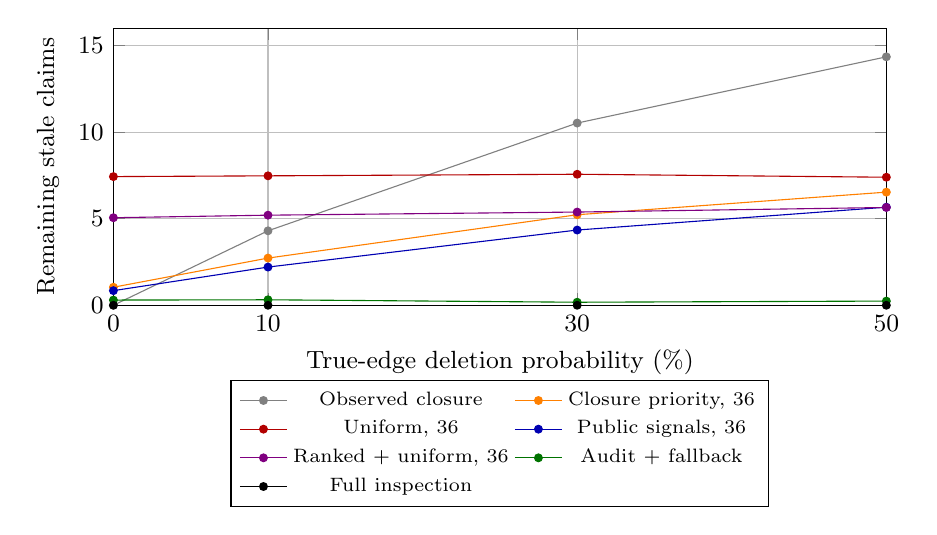
\begin{tikzpicture}\begin{axis}[width=0.94\linewidth,height=5.1cm,xlabel={True-edge deletion probability (\%)},ylabel={Remaining stale claims},xmin=0,xmax=50,ymin=0,ymax=16,xtick={0,10,30,50},grid=major,legend style={font=\scriptsize,at={(0.5,-0.27)},anchor=north,legend columns=2},label style={font=\small},tick label style={font=\small}]
\addplot[color=gray,mark=*,mark size=1.4pt] coordinates {(0,0.000000) (10,4.300000) (30,10.522222) (50,14.347222)};
\addlegendentry{Observed closure}
\addplot[color=orange,mark=*,mark size=1.4pt] coordinates {(0,1.041667) (10,2.725000) (30,5.227778) (50,6.533333)};
\addlegendentry{Closure priority, 36}
\addplot[color=red!70!black,mark=*,mark size=1.4pt] coordinates {(0,7.430556) (10,7.475000) (30,7.566667) (50,7.394444)};
\addlegendentry{Uniform, 36}
\addplot[color=blue!70!black,mark=*,mark size=1.4pt] coordinates {(0,0.844444) (10,2.205556) (30,4.344444) (50,5.663889)};
\addlegendentry{Public signals, 36}
\addplot[color=violet,mark=*,mark size=1.4pt] coordinates {(0,5.055556) (10,5.202778) (30,5.383333) (50,5.647222)};
\addlegendentry{Ranked + uniform, 36}
\addplot[color=green!45!black,mark=*,mark size=1.4pt] coordinates {(0,0.300000) (10,0.316667) (30,0.175000) (50,0.241667)};
\addlegendentry{Audit + fallback}
\addplot[color=black,mark=*,mark size=1.4pt] coordinates {(0,0.000000) (10,0.000000) (30,0.000000) (50,0.000000)};
\addlegendentry{Full inspection}
\end{axis}\end{tikzpicture}

\vspace{1.2cm}
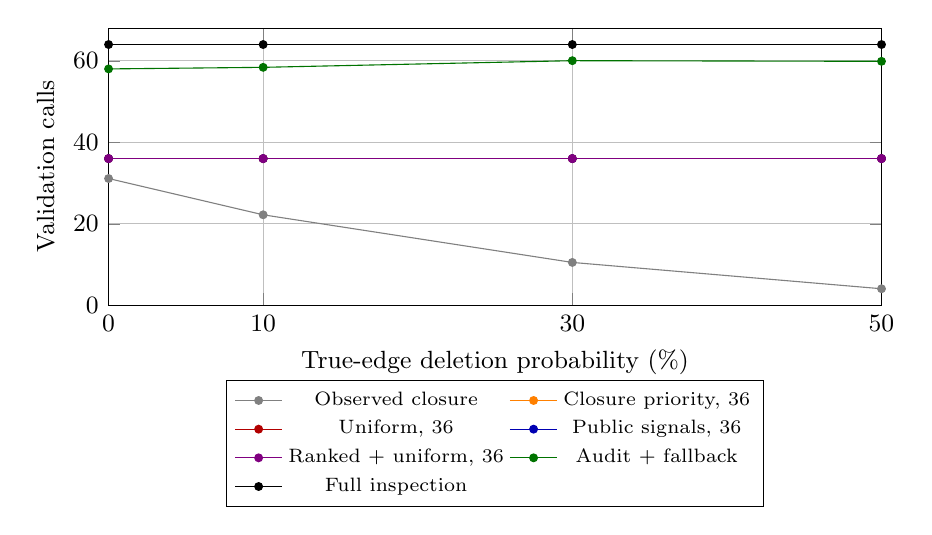
\begin{tikzpicture}\begin{axis}[width=0.94\linewidth,height=5.1cm,xlabel={True-edge deletion probability (\%)},ylabel={Validation calls},xmin=0,xmax=50,ymin=0,ymax=68,xtick={0,10,30,50},grid=major,legend style={font=\scriptsize,at={(0.5,-0.27)},anchor=north,legend columns=2},label style={font=\small},tick label style={font=\small}]
\addplot[color=gray,mark=*,mark size=1.4pt] coordinates {(0,31.108333) (10,22.205556) (30,10.513889) (50,4.052778)};
\addlegendentry{Observed closure}
\addplot[color=orange,mark=*,mark size=1.4pt] coordinates {(0,36.000000) (10,36.000000) (30,36.000000) (50,36.000000)};
\addlegendentry{Closure priority, 36}
\addplot[color=red!70!black,mark=*,mark size=1.4pt] coordinates {(0,36.000000) (10,36.000000) (30,36.000000) (50,36.000000)};
\addlegendentry{Uniform, 36}
\addplot[color=blue!70!black,mark=*,mark size=1.4pt] coordinates {(0,36.000000) (10,36.000000) (30,36.000000) (50,36.000000)};
\addlegendentry{Public signals, 36}
\addplot[color=violet,mark=*,mark size=1.4pt] coordinates {(0,36.000000) (10,36.000000) (30,36.000000) (50,36.000000)};
\addlegendentry{Ranked + uniform, 36}
\addplot[color=green!45!black,mark=*,mark size=1.4pt] coordinates {(0,58.011111) (10,58.400000) (30,60.033333) (50,59.877778)};
\addlegendentry{Audit + fallback}
\addplot[color=black,mark=*,mark size=1.4pt] coordinates {(0,64.000000) (10,64.000000) (30,64.000000) (50,64.000000)};
\addlegendentry{Full inspection}
\end{axis}\end{tikzpicture}

\vspace{1.2cm}
\caption{Measured residual claims and validation calls across missing-edge conditions; each point averages 360 generated base workspaces. Declining closure cost coincides with worse coverage. The audited policy includes its fallback cost. These are validator-call counts, not token or monetary savings.}\label{fig:missing}
\end{figure}

\begin{figure}[ht]
\centering
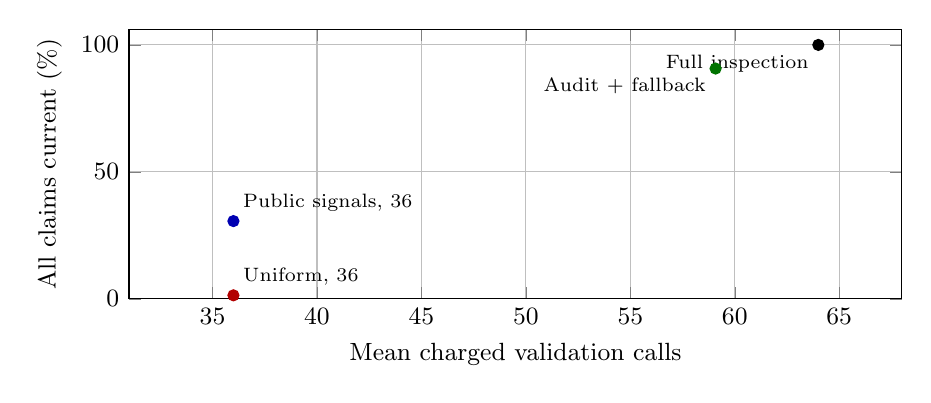
\begin{tikzpicture}\begin{axis}[width=0.94\linewidth,height=5cm,xlabel={Mean charged validation calls},ylabel={All claims current (\%)},xmin=31,xmax=68,ymin=0,ymax=106,grid=major,label style={font=\small},tick label style={font=\small}]
\addplot[only marks,color=red!70!black,mark=*,mark size=2pt] coordinates {(36.000000,1.388889)};
\node[above right,font=\scriptsize] at (axis cs:36.000000,1.388889) {Uniform, 36};
\addplot[only marks,color=blue!70!black,mark=*,mark size=2pt] coordinates {(36.000000,30.625000)};
\node[above right,font=\scriptsize] at (axis cs:36.000000,30.625000) {Public signals, 36};
\addplot[only marks,color=green!45!black,mark=*,mark size=2pt] coordinates {(59.080556,90.694444)};
\node[below left,font=\scriptsize] at (axis cs:59.080556,90.694444) {Audit + fallback};
\addplot[only marks,color=black,mark=*,mark size=2pt] coordinates {(64.000000,100.000000)};
\node[below left,font=\scriptsize] at (axis cs:64.000000,100.000000) {Full inspection};
\end{axis}\end{tikzpicture}
\caption{Selected policies illustrate the cost/correctness tradeoff. Audit plus fallback saves only 7.69\% of validation calls and has lower all-current frequency than full inspection. Its release tolerance explicitly allows nonzero residuals.}\label{fig:cost}
\end{figure}
\FloatBarrier

% END_AUTOGENERATED_RESULTS

\section{Practical interpretation for Manor}
The observed graph can prioritize work, but its completeness cannot be inferred from its own contents. A practical workspace controller needs to distinguish a heuristic candidate set from the condition under which other outputs may be reused. The study's gate makes that condition explicit, pays for additional validation and exposes fallback costs.

The inspected Manor implementation has source/version hashes, artifact-to-Knowledge associations and task-delivery checks. An eventual integration could attach a versioned observed-provenance record to each retained block and gate publication against a frozen source/target scope. This study does not implement that integration. It does not establish that current Manor can perform cross-artifact dependency repair, resolve semantic human conflicts or enforce the paper's count certificate in production.

\section{Limitations and publication status}
The main study is synthetic and uses an idealized exact validator and reference repairer. Its unit is a scalar claim block, not a complete document or an autonomous agent action. The families are parameterizations of a common generator and do not establish broad domain generalization. Random edge deletion and insertion do not substitute for natural extraction errors. Generator-conditioned lexical signals, free graph work, and perfect patches can overstate the practical value of selection.

The audit machinery is existing statistical methodology. Its guarantee is conditional on sampling, labels and snapshot stability; it controls a count and does not weight business severity. A small residual tolerance may be inappropriate for consequential outputs. Protecting separate note blocks is an API invariant shared by all policies, rather than a learned preservation capability. Complete-system methods, multiple models, actual generated repairs and independent human adjudication are outside the demonstrated main experiment.

This version is an openly released research preprint and executable prototype, not a journal acceptance or conference publication. The manuscript and code were prepared with AI assistance, including experiment scripting and independent automated review. Authorship and responsibility remain with the named author. No private application implementation, customer records, model credentials or prior patent submission materials are included in the release.

\clearpage
\section{Conclusion}
Selective repair requires checking what an observed graph can omit. The executable study separates value-changing obligations from graph reachability, compares matched validation budgets, and measures the price of a declared residual-count audit and fallback policy. It provides a reproducible boundary study for persistent workspaces. Establishing a competitive autonomous repair method requires natural extraction failures and end-to-end model repair evidence beyond this prototype.

\appendix
\section{Code and reproduction}
The artifact provides a dependency-free benchmark, frozen data, complete compressed traces, CSV summaries, tests, plotting code, manuscript source and PDF. From the repository root:
\begin{lstlisting}[language=bash]
python3 -B -m unittest discover -s code -p 'test_benchmark.py'
python3 -B code/benchmark.py sanity
python3 -B code/benchmark.py run --data-dir data \
  --out-dir results_reproduction --split test
\end{lstlisting}
The pre-existing frozen data must be reused for exact reproduction. Running the freeze command into a different empty directory regenerates the same canonical data and pins the exact code bytes. Changing code or protocol after freezing requires an explicitly new study version.

The core exclusion-bound implementation uses exact integer comparisons:
\begin{lstlisting}[language=Python]
denominator = comb(N, n)
tail = sum(comb(K, x) * comb(N-K, n-x)
           for x in range(max(0, n-N+K), min(k,n,K)+1))
admissible = tail * delta.denominator > \
             denominator * delta.numerator
\end{lstlisting}
The full code in \texttt{code/benchmark.py} implements monotone inversion, public-only selection, exact validation accounting and the one-look gate. No tool output, source hash or confidence interval is a substitute for testing the assumptions of a production validator.

\begin{thebibliography}{9}
\bibitem{codeplan} R. Bairi et al. \emph{CodePlan: Repository-level Coding using LLMs and Planning}. FSE 2024. \url{https://arxiv.org/abs/2309.12499}.
\bibitem{ledger} H. Wang et al. \emph{LEDGER: Scaling Agentic Document Editing with Dependency-aware Graph Retrieval}. Findings of ACL 2026. \url{https://aclanthology.org/2026.findings-acl.515/}.
\bibitem{memorepair} \emph{MEMOREPAIR: Barrier-First Cascade Repair in Agentic Memory}. arXiv:2605.07242, 2026. \url{https://arxiv.org/abs/2605.07242}.
\bibitem{boardroom} S. Manivannan. \emph{BoardroomAI: Dependency-Aware Human-Steerable Multi-Agent Deliberation through Evolving Decision Graphs}. arXiv:2608.13046, 2026. \url{https://arxiv.org/abs/2608.13046}.
\bibitem{cavert} Z. Yu et al. \emph{Beyond Corrected Memory: Execution Consistency in Multi-Agent Systems}. arXiv:2610.08101, 2026. \url{https://arxiv.org/abs/2610.08101}.
\bibitem{coverage} \emph{Finite-Sample Coverage Audits for High-Recall Candidate Generation: Certification and Learning-Theoretic Design}. arXiv:2607.21480, 2026. \url{https://arxiv.org/abs/2607.21480}.
\bibitem{selective} \emph{Exact Finite-Population Sequential Auditing for Selective Release from Model-Proposed Candidate Sets}. Mathematics 14(18), 3427, 2026. \url{https://doi.org/10.3390/math14183427}.
\end{thebibliography}
\end{document}
